\section*{Task 2: XSS and CSRF}
\subsection*{Exercises:}
\begin{enumerate}
\item The steps are as follows: 
  \begin{itemize}
  \item Open BadStore in your browser.
  \item Click "Sign Our GuestBook" on the left side of the page.
  \item In the "Your Name" field, type whatever you want.
  \item In the "Email" field, type whatever you want.
  \item In the "Comments" field, type \textit{<script>alert("1")</script>} .
  \item Click "Add Entry", the page should like this below:
  \end{itemize}
  \begin{figure}[h!]
    \caption{Alert Made by XSS Attack}
    \begin{center}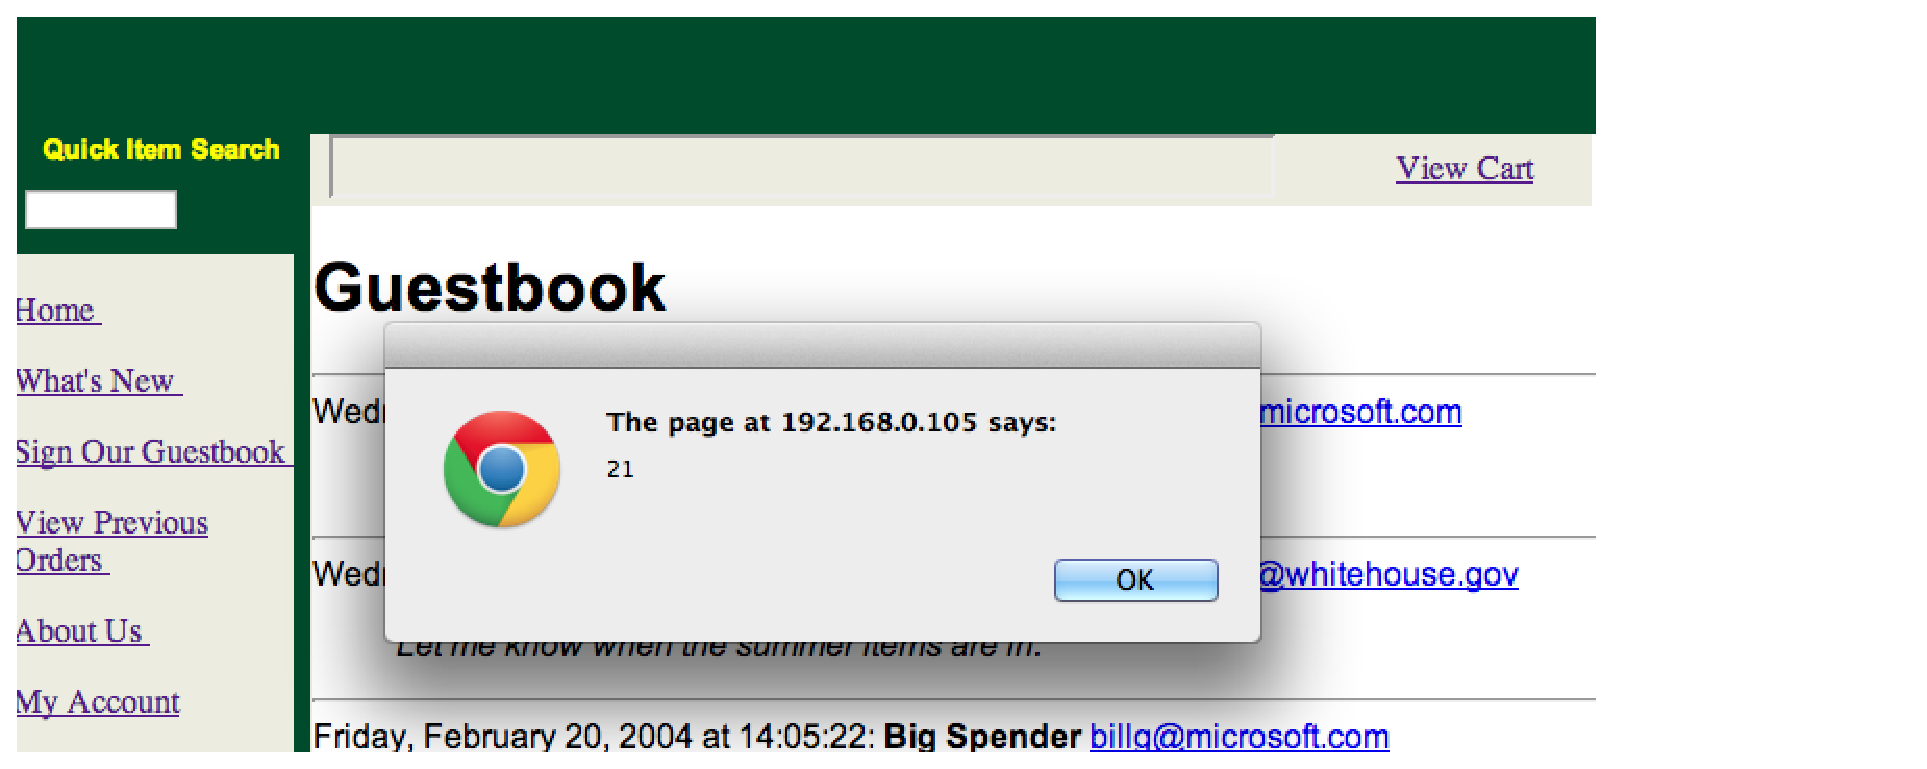
\includegraphics[height=2.5in]{xss}
    \end{center}
  \end{figure}

  Explanation: In the example, we write a piece of Javascript code enclosed in script tags in the comment area and submit it to the guest book. It works because the website has an XSS vulnerability which enables us to insert Javascript into the website and have it executed by other users. When the page reloads, the server will just paste the tag-embraced Javascript code into the HTML code in such a way that it is interpreted as a Javascript snippet rather than the text \verb|<script>alert("1")</script>|.
\item To perform a CSRF attack, we need to create a custom web page containing deceptive information. The objective of the attack is to have an unsuspecting user make an XSS comment in the guestbook for generating countless alert messages. The key point necessary to execute the attack is to guide the victim to our page and have him or her click on the button. As we demonstrate it just as an example, we can suppose that the victim will click on it. The custom page is so simple that it is just written as a demo. Below are the steps for carrying out the attack:
  \begin{itemize}
  \item As the attacker, write a simple page containing this code:
    \par
    \begin{lstlisting}[language=HTML,numbers=left,numberstyle=\tiny,columns=fullflexible,basicstyle=\footnotesize\ttfamily]
      <!DOCTYPE html>
      <html>
      <head>
      <title>iPhone Free!</title>
      </head>
      <body>
      <FORM METHOD="POST" ACTION="http://10.0.2.5/cgi-bin/badstore.cgi?action=doguestbook">
      <INPUT TYPE=hidden NAME=name value="<script>for(var i=0;i<10000;i++){alert('HHHH');}</script>" SIZE=30>
      <INPUT TYPE=hidden NAME=email value="1" SIZE=40>
      <TEXTAREA style="display:none" NAME=comments COLS=60 ROWS=4 value="aaa"> </TEXTAREA>
      <INPUT TYPE=submit VALUE="Get Now!">
      <INPUT style="display:none" TYPE=reset></Center>
      </FORM>
      </body>
      </html>
    \end{lstlisting}
  \item The page shows like this:
    \begin{figure}[h!]
      \caption{Fake Page}
      \begin{center}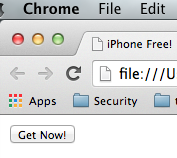
\includegraphics[height=2.5in]{csrf1}
      \end{center}
    \end{figure}
  \item As the victim, open BadStore and log in as a user.
  \item Visit the malicious page and click the "Get Now!" button.
  \item The victim will then be redirected into BadStore, as is shown in \autoref{fig:csrfVictim}.
    \begin{figure}[h!]
      \caption{Result after Performing CSRF Attack}
      \label{fig:csrfVictim}
      \begin{center}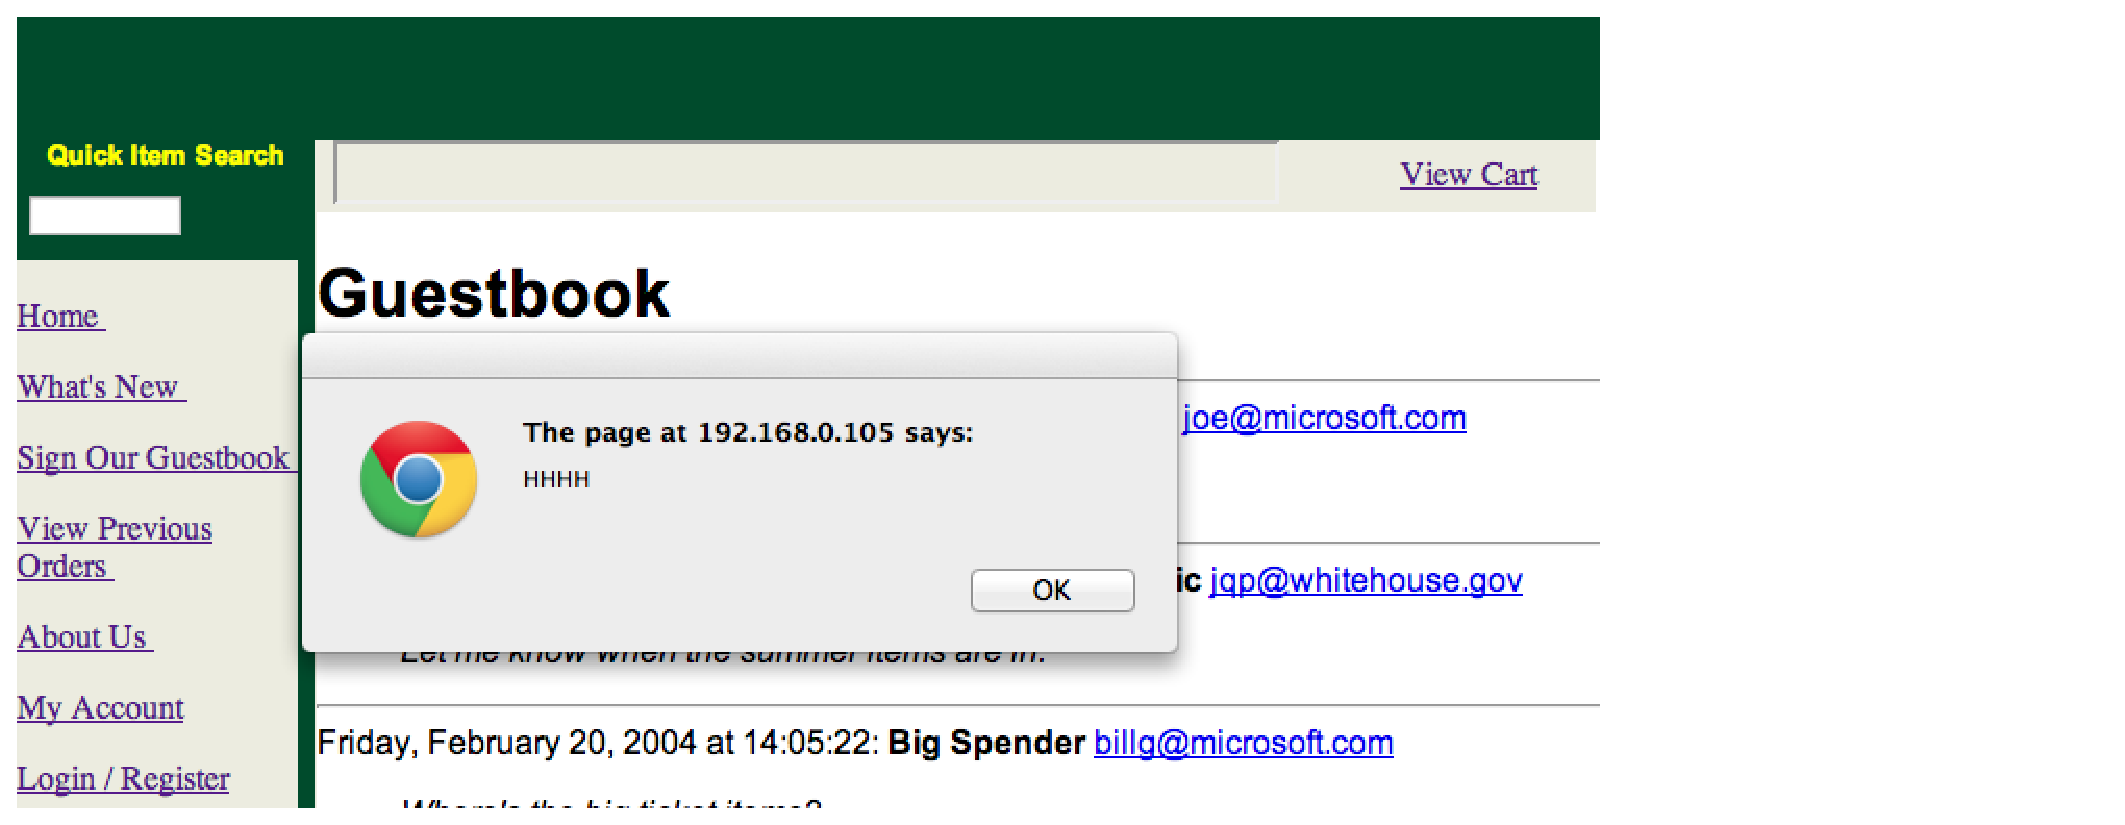
\includegraphics[height=2.5in]{csrf2}
      \end{center}
    \end{figure}
  \item The alert will repeat again and again as well as leaving many comments.
  \item Note: There might be some different performance in different browsers. i.e. Safari will operate the code after you quit it and reopen it.
  \end{itemize}
  \indent Explanation: In the example, we use a self-written page to perform the CSRF attack. As mentioned above, the key point is that the attacker needs to persuade the victim to visit the deceived page which contains the evil code. The code works as follows: The code sends a request to the server (BadStore), which could be as serious as submitting an order or transferring money to another account; and it works if the victim does not close the server website. To make it clear, the cookie of the server website still exists in the browser. As a result, when the server receives the deceived request, it will think that the request is made by the victim and perform the related operation.
\item The difference is that, in an XSS attack, the attacker makes the attack by inserting Javascript code (or other code) into the site. Because the site does not have strict checks on user inputs, the code can be planted into HTML and executed when the page is loaded. On the contrary, CSRF attacks do not necessarily need Javascript \cite{website:wikipedia_CSRF_XSS}. The most important part is that the attacker must acquire trust from the user and have him operate the deceived request. Also, the user cannot quit the page because the code will only work when the cookie of the target page stays in the browser. It is not the attacker himself that makes it work.
\item \highergradesonly
\item \highergradesonly
\end{enumerate}
